\documentclass[12pt]{article}
\usepackage{setspace}
\usepackage[margin=0.8in]{geometry}
\usepackage{url}
\usepackage{graphicx}
%\usepackage{comment}
%\doublespacing
%\usepackage[backend=biber]{biblatex}
%opening
%\addbibresource{master.bib}
\doublespacing
\title{\textbf{Kernel Organization}}
\author{Adam Sumner}
\date{February 1st, 2015 }

\begin{document}
%\twocolumn

\maketitle
\thispagestyle{empty}

\twocolumn
\setcounter{page}{1}
\iffalse \begin{abstract}
	This paper will address three types of kernel implementations: the monolithic kernel, the microkernel, and the exokernel. First, the general functionality of a kernel will be explored. The three implementation will then be analyzed, operating systems utilizing these implementations will be explored, and an argument will be presented to determine which of the three designs is the best choice for a modern, general purpose operating system.
\end{abstract}
\fi
\section{Kernel Overview}\label{sec:kernel}
\subsection{The Kernel}
In computing, the kernel is a computer program that manages input/output requests from software and translates them into data processing instructions for the central processing unit and other electronic components of a computer\cite{OS}. It acts as a link between user/system applications and the hardware that is physically installed in the system. This allows it to manage the system's resources. It is also able to provide the lowest level of abstraction for the resources that any software application may need to perform its respective function. Because of the critical functionality that it provides, it is considered to be the most important part of any OS. 

In general, Operating Systems are split into two separate parts: the user space, and the kernel space. Without this distinction, it would be impossible to provide a layer of protection for critical processes that keep the system stable. Depending on the kernel implementation, what actually resides in each respective space differs.
\subsection{The Monolithic Kernel}
The Monolithic Kernel is an OS architecture where the entire operating system is located in the kernel space\cite{Mono}, while applications and libraries are left to reside in user space. What this means is that I/O, virtual memory, VFS, device drivers, scheduling, memory allocation, etc., are a tight group that shares the same space in the OS. This enables the kernel developer to produce a singular piece of software that manages all of the low layer abstractions for the functionality of the entire system. Furthermore, the design is simple compared to other types of kernel implementations. It is one single binary file that can invoke functions directly. This can be shown in Figure \ref{fig:monolithic}.

\begin{figure}[h!]
\centering
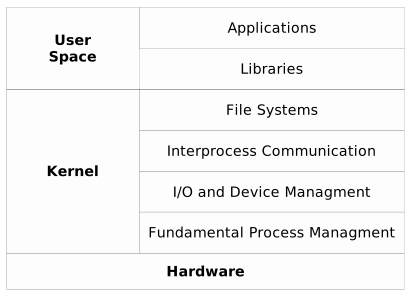
\includegraphics[width=\linewidth]{pictures/monolithic}
\caption{Monolithic Kernel Overview\cite{Vs}}
\label{fig:monolithic}
\end{figure}


Because the kernel is responsible for all of the basic services of the operating system, the source is a lot smaller than other implementations. What this means is that when compiled, since it is one file, the binary is much smaller, allowing the OS to perform faster. Furthermore, having one location for the entire system means that there are expected to be less bugs, along with a reduced amount of security issues. 

Unfortunately there are some drawbacks that come with utilizing a monolithic kernel. Even though the kernel is one file which lets the system perform faster, the actual source contains millions of lines of code. Moreover, this makes maintenance becomes difficult to deal with. This is because every time a bug is encountered and fixed, the entire source must be recompiled. Not only this, but the developer must first find the chunk within the pile of code that pertains to the issue. It could be compared to finding a needle in a haystack. This becomes a major issue concerning both time and resources.
\subsection{The Microkernel}
The Microkernel or $\mu$-kernel is a completely different approach to its monolithic predecessor. The core idea behind the $\mu$-kernel is to reduce the kernel as much as possible: \emph{Less is More}. The kernel is designed to handle only the necessary functions of an operating system, while the rest of the system services reside in the user space. This is shown in Figure \ref{fig:microkernel}.

\begin{figure}[h!]
\centering
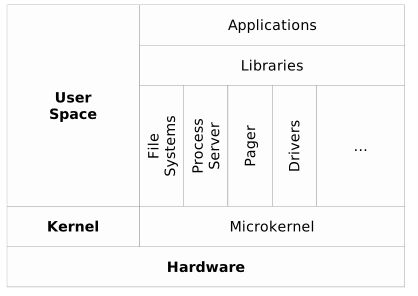
\includegraphics[width=\linewidth]{pictures/microkernel}
\caption{MicroKernel Overview\cite{Vs}}
\label{fig:microkernel}
\end{figure}

It is clear by comparing Figures \ref{fig:monolithic} and \ref{fig:microkernel} that they can be considered polar opposites of eachother. The $\mu$-kernel was designed to overcome the disadvantages that were the result of using a monolithic kernel. But how is the $\mu$-kernel able to handle all of the system services when it is not directly in charge of them? This is done through the idea of something known as ``context switches''. There is a server for each functionality such as managing memory issues, process management, etc\cite{wiki:micro}. Because these servers are not running in kernel space, ``context switching'' allows the user processes to enter a privileged mode in order to access the required resources. This is the core concept that enables the $\mu$-kernel design to work. The $\mu$-kernel truly becomes a middle man because the kernel is no longer a block of system services, as seen in the monolithic approach. It now represents several basic abstractions and primitives to control communication between processes and between a process and the underlying hardware. Because communication is done directly from the kernel to the system services, a message system is introduced which allows independent communication and favors extensibility\cite{Vs}. This is the key advantage of using a $\mu$-kernel design, extensibility. If new OS functionality is needed, rather than having to add it to the single piece of code and recompile the entire kernel as with a monolithic system, a new server can simply be added. Furthermore, the sheer size of the kernel is greatly reduced(consisting of roughly 10,000 lines of code) so maintenance on the kernel is a great ton easier than trying to edit/search through millions of lines of code as with a monolithic implementation. 

Of course this kernel design is no Mary Sue. While the $\mu$-kernel is minimalistic, easily updated, and implements strong protection of the system, the major drawback is performance.\\While previously the monolithic kernel can call all of its functions directly, ``context switching", though enabling the $\mu$-kernel design to work, comes at a high cost of overhead. To exemplify this, consider the monolithic kernel. A service only requires two mode switches(changes of the processor's ring or CPU mode). However, in a $\mu$-kernel based system, a service is obtained by sending an IPC message to a server, and obtaining the result in another IPC message from the server. In addition, passing the actual data to the server and back may include some extra copying overhead, while in a monolithic system, the kernel has direct access\cite{wiki:micro}. It should be noted that even though the $\mu$-kernel improved upon the monolithic kernel in many ways, it did this at the cost of its own performance. 
\subsection{The Exokernel}
The exokernel is an OS that was developed at MIT by the Parallel and Distributed Operating Systems group. Its main focus is to eliminate the notion that an OS should provide abstractions on which applications are built. It concentrates solely on securely multiplexing the hardware, meaning application-level libraries and servers can directly implement OS abstractions\cite{MIT}. What this allows applications to do is to essentially communicate directly with the hardware. This gives more control to the application developer because the exokernel only provides basic low level abstractions, while the application will define its own abstraction of the hardware, if need be. This is shown in Figure \ref{fig:exokernel}.

\begin{figure}[h!]
\centering
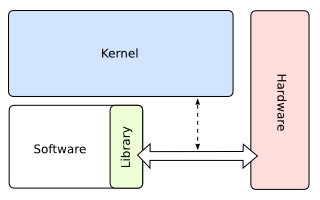
\includegraphics[width=\linewidth]{pictures/exokernel}
\caption{Exokernel Overview\cite{exo}}
\label{fig:exokernel}
\end{figure}

 For example, the kernel will prevent basic unauthorized reading/writing to memory, but the individual application will decide how memory is actually abstracted. The advantage to using an exokernel is that kernel source code is of the most basic form. As a result, it does not impose high level abstractions, like the $\mu$-kernel does, on its user applications. On the one hand, programmers can be extremely efficient with their software, however on the other, it's necessary to write a library for each application on the system, whereas in the other designs, this library is already implemented by the kernel. It has the potential to create a truly optimized machine, however, this is solely dependent on those who develop software for the system. Where it excels in the freedom it gives developers on hardware abstractions and efficiency, only those who are truly dedicated will even bother to develop software for these systems. This is its major flaw. It is a great theoretical concept to let programmers define their own hardware abstractions, but why reinvent the wheel?

\section{OS Kernel\\ Implementations}\label{sec:OS}
\subsection{Linux/Unix}
The most popular Operating System that utilizes a monolithic kernel and is widely used today, is Linux. Linux was developed by Linus Torvalds in 1991 and is considered to be a Unix-like OS. The impact of his choice to implement a monolithic kernel has gotten Mr. Torvalds into some heated debates, however, twenty-four years later, development is in full swing and hasn't adversely affected the systems growth in any major way. Currently, the kernel has evolved into a modular system. This means that even though the kernel is still monolithic, it doesn't have to load everything at boot time, and if a new module is needed, it isn't necessary to recompile the entire kernel. Choosing to use a monolithic kernel was an appropriate choice because $\mu$-kernel systems were relatively new, and Linus based his system on what he had studied in his Operating System classes(UNIX) at the University of Helsinki.
\subsection{Minix}
It almost goes without saying that if Linux is mentioned in this paper, Minix is a must. This OS was developed by Andrew S. Tanenbaum, a professor at the VU University Amsterdam, and it utilizes the $\mu$-kernel. At this time, it was clear that the $\mu$-kernel was an improvement on the monolithic approach, and being a research professor, it only makes sense that he would choose this kernel for his system. His design choice, in my opinion, was detrimental to the popularity of Minix vs Linux's popularity because it wasn't as portable. The $\mu$-kernel was fairly new and didn't have as much history as the monolithic kernel, so its functionality was definitely lacking, but pioneers are never the ones who perfect their discoveries.

\subsection{Aegis/XOK}
Aegis was the first exokernel OS to be developed. It was created for the proof of concept of the exokernel design. It was an appropriate kernel choice clearly because it was designed to support the fact that exokernels are in fact a feasible approach to kernel design. It featured little storage support, and XOK, the successor, was then developed. It was able to apply the exokernel concept more thoroughly than Aegis and is MIT's current version of the exokernel.  However, the exokernel design is such a new and system specific design that commercially, it will not become a popular approach in the near future outside of research.
\section{The ``Best" Choice}
Based on the information presented in Sections \ref{sec:kernel} and \ref{sec:OS}, it should be clear that the $\mu$-kernel is the most advantageous kernel design to utilize.
It beats the monolithic both in extensibility and maintenance. These two features are the most important when designing a system to be the best it can possibly be. Furthermore, the exokernel, while extremely similar to the $\mu$-kernel, still does not come up to par with it. This is because it is a kernel designed for extremely specific purposes. When concerning a modern, general purpose operating system, the amount of applications that would need to implement their own libraries for hardware abstractions would be tremendous. The $\mu$-kernel provides all the advantages of the exokernel without any of its drawbacks. Performance wise, one could argue that the monolithic kernel wins, but with rapid improvement of processing power in such a short amount of time(Moore's Law), this becomes an unnoticeable difference for the generic user.


\singlespacing
\bibliographystyle{plain}
\bibliography{master}


\end{document}
